\section{OTP}

	\begin{frame}
		\begin{center}
			\LARGE{\textcolor{blue}{Il cifrario perfetto: One-Time Pad}}
		\end{center}
	\end{frame}

	\subsection{Cifrari perfetti}
	
	{
		\fontsize{10}{0}
		\begin{frame}
			\frametitle{I cifrari perfetti}
			Siano $P,K,C$ \tblue{variabili aleatorie} su insiemi finiti di valori
			\begin{center}
				$\begin{cases}
					P \text{ prende valori nell'insieme dei plaintext}\\
					K \text{ prende valori nell'insieme delle chiavi}\\
					C \text{ prende valori nell'insieme dei ciphertext}
				\end{cases}$
			\end{center}
			Supponiamo $P$ e $K$ \tblue{indipendenti}.
			\begin{block}{}
				Un cifrario si dice \tblue{perfetto} se
				$$\forall p \in P \text{ e }\forall c \in C \text{ con } Pr(C=c) > 0 \text{ vale che:}$$
				$$Pr(P=p|C=c) = Pr(P=p)$$
			\end{block}
		\end{frame}
	}
	\begin{frame}
		\frametitle{One Time Pad}
		\begin{columns}
			\begin{column}{0.4\textwidth}
				\begin{center}
					\begin{figure}
						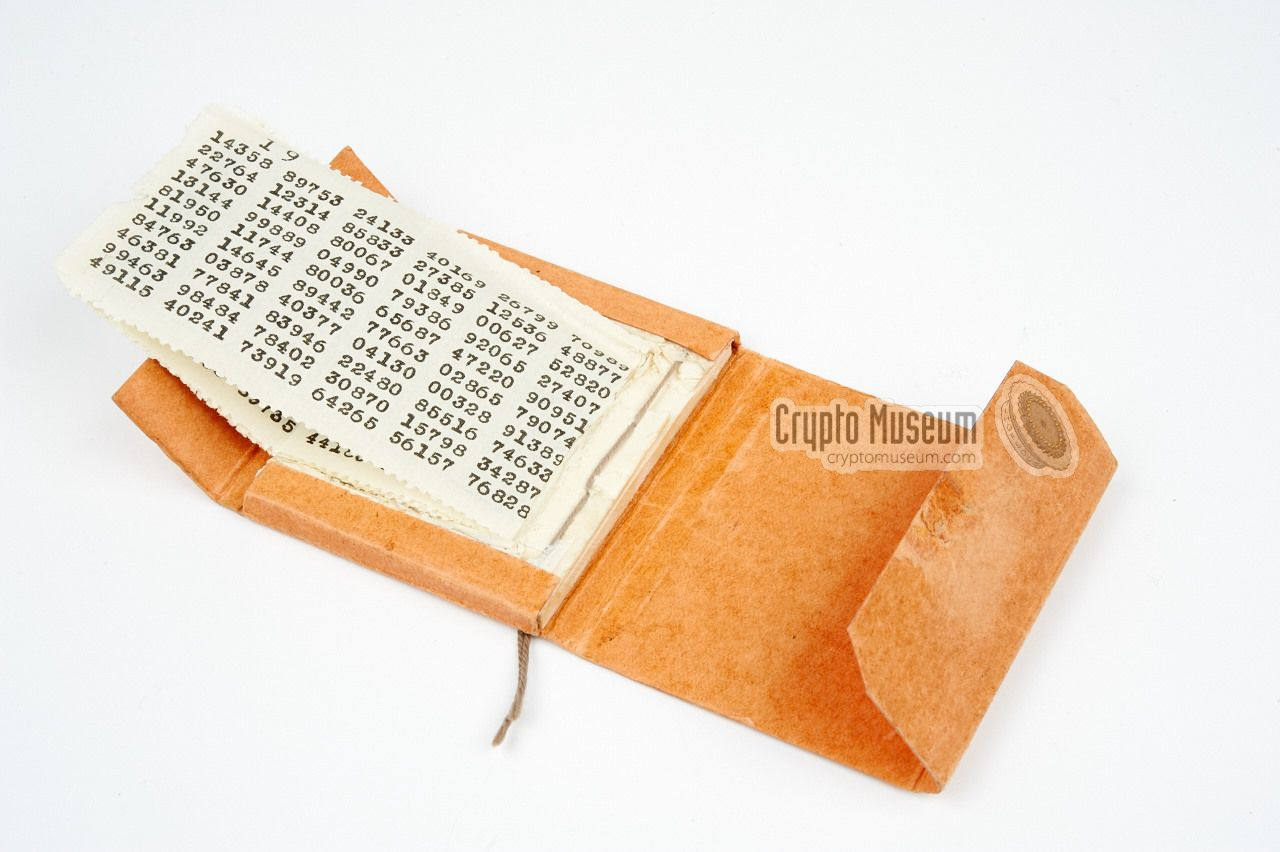
\includegraphics[width=\columnwidth]{img/otp.jpg}
						\caption{One Time Pad sovietico}
					\end{figure}
				\end{center}
			\end{column}
			\begin{column}{0.6\textwidth}
				\begin{itemize}
					\item Introdotto dall'ingegnere dei Bell Labs, \tblue{Gilbert Sandford Vernam} (1890 – 7 febbraio 1960), nel 1926
					\item Il nome deriva dai \tblue{blocchetti} su cui venivano scritte le chiavi
					\item Fissiamo $P = C = K = \{0,1\}^N \text{ con } N>0\text{ \tblue{fissato} e \tblue{noto}}$
					\item Chiave \tblue{perfettamente} casuale $\Rightarrow Pr(K=k)=\frac{1}{2^N}$
				\end{itemize}
			\end{column}
		\end{columns}
	\end{frame}

	\begin{frame}
		\frametitle{One Time Pad}
		Le funzioni di Encryption e di Decryption sono definite come segue:
		$$\begin{cases}
			E_k[p] = p \oplus k = c\\
			D_k[c] = c \oplus k = p \oplus k \oplus k = p
		\end{cases}$$
		{
			\fontsize{10}{0}
			\begin{block}{Esempio}
				$N = 4, P=K=C=\{0,1\}^4$ e supponiamo che i possibili plaintext siano $(0101)$ con probabilità $\frac{3}{4}$ e $(1011)$ con probabilità $\frac{1}{4}$. Se viene scelto $p = (0101) \ e\ k = (1100)$ (che ha probabilità $\frac{1}{2^4}$) otteniamo  $E_k[p] = p \oplus k = (1001) = c$. Lo stesso $c$ è però ottenibile con l'altro $p = (1011)$ e $k = (0010)$. Osservare $c$ come ciphertext non ci permette di risalire con certezza a $p$ senza conoscere $k$.
			\end{block}
		}
	\end{frame}

	\subsection{Dimostrazione}

	\begin{frame}
		\frametitle{One Time Pad}
		\begin{block}{OTP è un cifrario perfetto}
			Supponiamo che ogni $p$ abbia probabilità non nulla di essere generato. Sia $p\in P \ e\ c \in C$ rispettivamente un plaintext e un ciphertext qualsiasi di probabilità non nulla. Dobbiamo dimostrare che $$Pr(P=p|C=c) = Pr(P=p)$$
		\end{block}
	\end{frame}
	\begin{frame}
		\frametitle{One Time Pad}
		$$Pr(P=p|C=c) = \frac{Pr(C=c|P=p)Pr(P=p)}{Pr(C=c)}$$
		Visto che $c = p \oplus k \Leftrightarrow k = c\oplus p$ vuol dire che esiste una \emph{e una sola} chiave $k_{m,c} = c \oplus p$ che permette di cifrare $p$ in $c$ e quindi $$\forall p,c$$ vale che $$Pr(C=c|P=p) = Pr(k_{m,c}) = \frac{1}{2^N}$$ per la distribuzione uniforme delle chiavi.
	\end{frame}
	\begin{frame}
		\frametitle{One Time Pad}
		$$Pr(P=p|C=c) = \frac{\frac{1}{2^N}Pr(P=p)}{Pr(C=c)}$$
		Calcoliamo $Pr(C=c)$ come segue:
		\begin{align*}
			Pr(C=c) &= \sum_{p'\in P}^{}Pr(C=c|P=p')Pr(P=p')\\
			&= \sum_{p'\in P} \frac{1}{2^N}Pr(P=p')\\
			&=\frac{1}{2^N}\sum_{p'\in P}Pr(P=p')\\
			&= \frac{1}{2^N}
		\end{align*}
	\end{frame}
	\begin{frame}
		\frametitle{One Time Pad}
		Da cui si ottiene:
		$$Pr(P=p|C=c) = \frac{\cancel{\frac{1}{2^N}}Pr(P=p)}{\cancel{\frac{1}{2^N}}} = Pr(P=p)$$
	\end{frame}
	\begin{frame}
		\frametitle{Ma allora perché non si usa?}
		\begin{itemize}
			\item Chiave lunga tanto quanto il messaggio
			\item Scala difficilmente con un grande numero di nodi
			\item Sequenze di bit realmente casuali sono difficili da generare
			\item Si stanno studiando metodi quantistici di generazione e distribuzione di chiavi
		\end{itemize}
	\end{frame}
